\subsection{Home Range Detection}
A total of 908 years of data stemming from 309 individuals met the requirements for conducting a home range detection. The validation data shows that out of these 908 cases, in 49\% (441) of all cases there was a settlement in a home range and in 51\% (467) of all cases there was no settlement in a home range.

After performing the home range detection, a home range was predicted for 69\% (626) of all cases. Based on the validation data, 429 out of these 626 actually had a home range, while 197 did not have a home range (Table~\ref{table:conf_matrix_hr}). Thus, 69\% (429 out of 626) of the positively predicted cases were correctly predicted. For 31\% (282) of all cases, no home range was predicted. Based on the validation data, 270 out of these 282 actually had no home range, while 12 did have a home range. Thus, 96\% (270 out of 282) of the negatively predicted cases were correctly predicted. Overall, 77\% (699 out of 908) of the cases could be correctly predicted, resulting in an accuracy of 77\%. While a value of 97\% was achieved for recall, the precision is 69\% and MCC is 60\% (Table~\ref{table:stats_hr_and_nest}).

\begin{table}[H]
\begin{center}
\caption[Confusion matrix of the home range detection result]{Confusion matrix of the home range detection result.}
\label{table:conf_matrix_hr}
\begin{tabularx}{0.5\textwidth} {
    | >{\centering\arraybackslash}X 
    | >{\centering\arraybackslash}X 
    | >{\centering\arraybackslash}X | }
\hline
Total \break = 908 & \textbf{Predicted \break positive} & \textbf{Predicted \break negative} \\
\hline
\textbf{Actually \break positive} &
\cellcolor[HTML]{CCFFCC} TP = 429 \break (47.3\%) & % green
\cellcolor[HTML]{FFCCCC} FN = 12 \break (1.3\%) \\  % red
\hline
\textbf{Actually \break negative} &
\cellcolor[HTML]{FFCCCC} FP = 197 \break (21.7\%) &  % red
\cellcolor[HTML]{CCFFCC} TN = 270 \break (29.7\%) \\ % green
\hline
\end{tabularx}
\end{center}
\end{table}

The differences between the two categories (whether a home range was occupied or not) and both sexes are shown in Figure~\ref{figure:hr_area_centroid_displacement_sex_diff}. The differences were analysed statistically using a t-test. With a p-value of < 2.2$\times10^{-16}$, the category with home range shows a significantly higher number of consecutive weeks spent in an area of less than 60 km$^2$ than the category without home range. There is also a difference between both sexes for the cases where a home range was present with a p-value of 0.02, indicating that male individuals tend to spend more consecutive weeks in an area of less than 60 km$^2$. Regarding the centroid displacement between the respective areas, a p-value of < 2.2$\times10^{-16}$ shows that the cases without a home range have a significantly higher centroid displacement than the cases with a home range. There is, however, no significant difference between the two sexes for cases where a home range was present is with a p-value of 0.48.

\begin{figure}[H]
\centering
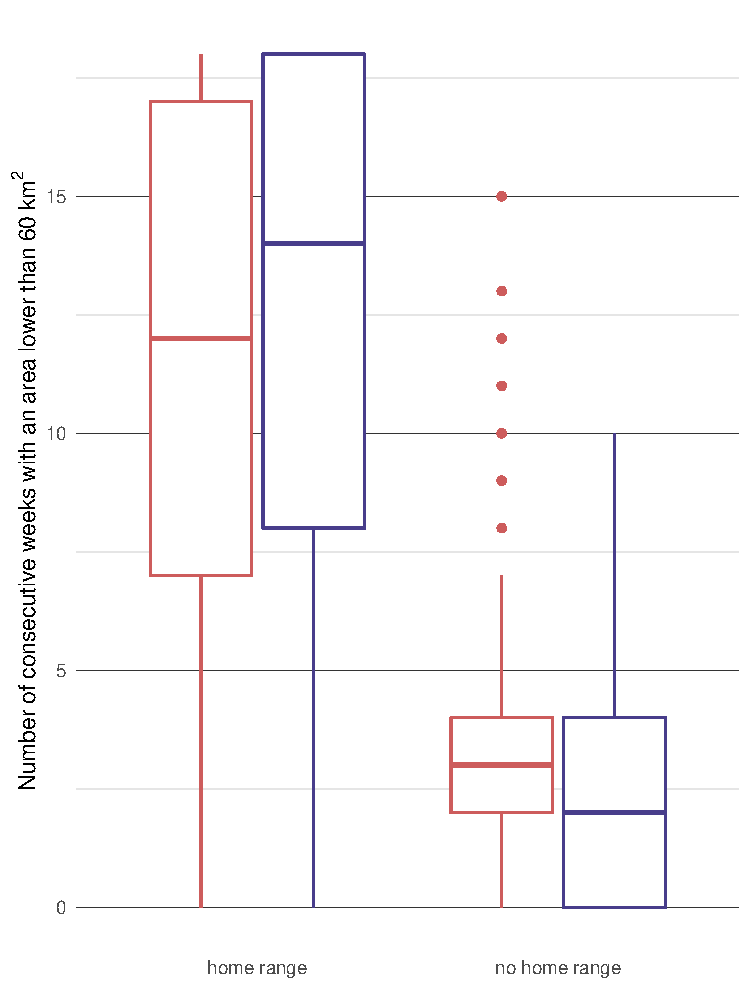
\includegraphics[width=0.4\textwidth]{figures/results/02_hr_area_sex_diff_no_legend.pdf}
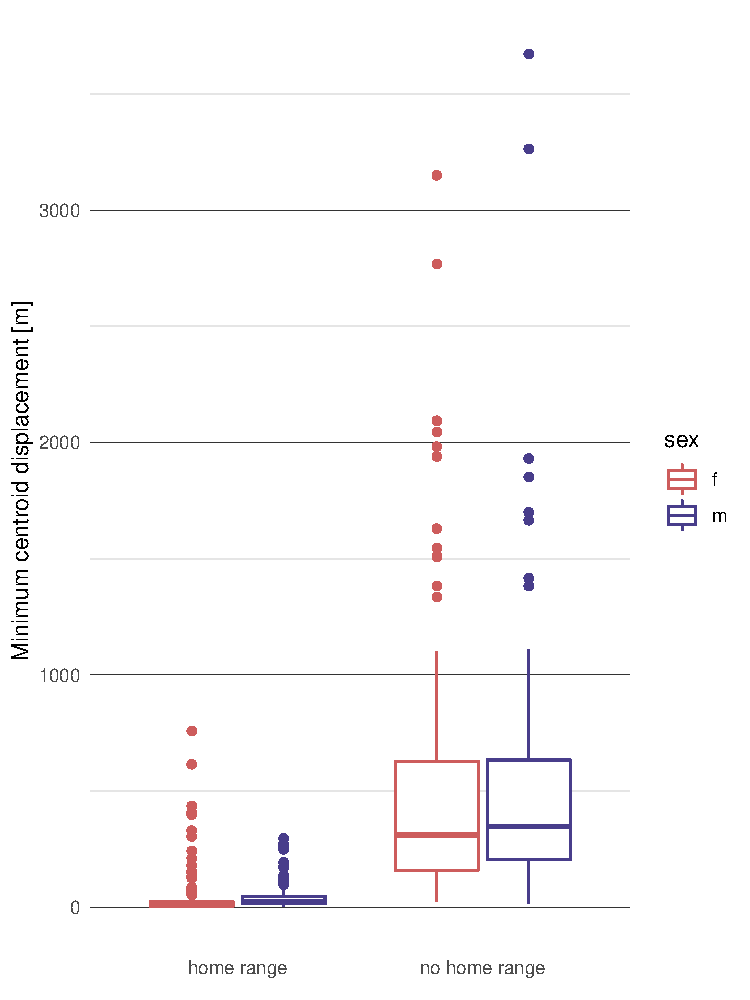
\includegraphics[width=0.4\textwidth]{figures/results/04_centroid_displacement_sex_diff.pdf}
\caption[Boxplot of birds with and without home range]{The boxplots show the difference in consecutive weeks with an area usage of < 60km$^2$ (left) and minimum centroid displacement between consecutive MCPs (right) for female (red) and male (blue) individuals with and without a home range according to the validation data.}
\label{figure:hr_area_centroid_displacement_sex_diff}
\end{figure} 


\subsection{Nest Detection}
The 626 positively predicted cases of the previous step were considered for nest detection analyses. Out of these 626 cases, 624 met the minimum data requirements to perform a nest detection analysis. The validation data shows that out of these 624 cases, in 58\% (365) of all cases a nest was occupied and in 42\% (259) of all cases no nest was detected in field observations.

After performing the nest detection, a nest was predicted for 70\% (437) of all cases. Based on the validation data, 364 out of these 437 actually had a nest, while 73 did not have a nest (Table \ref{table:conf_matrix_nest}). Thus, 83\% (364 out of 437) of the positively predicted cases were correctly predicted. For 31\% (187) of all cases, no nest was detected. Based on the validation data, 186 out of these 187 actually had no nest, while 1 did have a nest. Thus, 99\% (186 out of 187) of the negatively predicted cases were correctly predicted.  Overall, 88\% (550 out of 624) of the cases could be correctly predicted, resulting in an accuracy of 88\%. While a value of 99\% was achieved for recall, the precision is 83\% and MCC is 77\% (Table~\ref{table:stats_hr_and_nest}).

\begin{table}[H]
\begin{center}
\caption[Confusion matrix of the nest detection result]{Confusion matrix of the nest detection result.}
\label{table:conf_matrix_nest}
\begin{tabularx}{0.5\textwidth} {
    | >{\centering\arraybackslash}X 
    | >{\centering\arraybackslash}X 
    | >{\centering\arraybackslash}X | }
\hline
Total \break = 624 & \textbf{Predicted \break positive} & \textbf{Predicted \break negative} \\
\hline
\textbf{Actually \break positive} &
\cellcolor[HTML]{CCFFCC} TP = 364 \break (58.3\%) & % green
\cellcolor[HTML]{FFCCCC} FN = 1 \break (0.2\%) \\  % red
\hline
\textbf{Actually \break negative} &
\cellcolor[HTML]{FFCCCC} FP = 73 \break (11.7\%) &  % red
\cellcolor[HTML]{CCFFCC} TN = 186 \break (29.8\%) \\ % green
\hline
\end{tabularx}
\end{center}
\end{table}

The differences between the two categories (whether a nest was present or not) and both sexes are shown in Figure~\ref{figure:res_time_revisits_sex_diff}. The differences were analysed statistically using a t-test. With a p-value of < 2.2$\times10^{-16}$, the category with a nest shows a significantly higher mean daily residence time at the calculated nest location than the category without a nest. Also, the difference between the two sexes for cases where a nest was present is significantly higher with a p-value of < 2.2$\times10^{-16}$, indicating that female red kites tend to spend significantly more time at the nest. Regarding the mean daily revisitations to the calculated nest location, a p-value of < 2.2$\times10^{-16}$ shows that the cases with a nest have a significantly higher revisitation rate than the cases without a nest. The difference between the two sexes for cases where a nest was present is also significant with a p-value of < 2.2$\times10^{-16}$. Female individuals tend to revisit the calculated nest location significantly more than male individuals.

\begin{figure}[H]
\centering
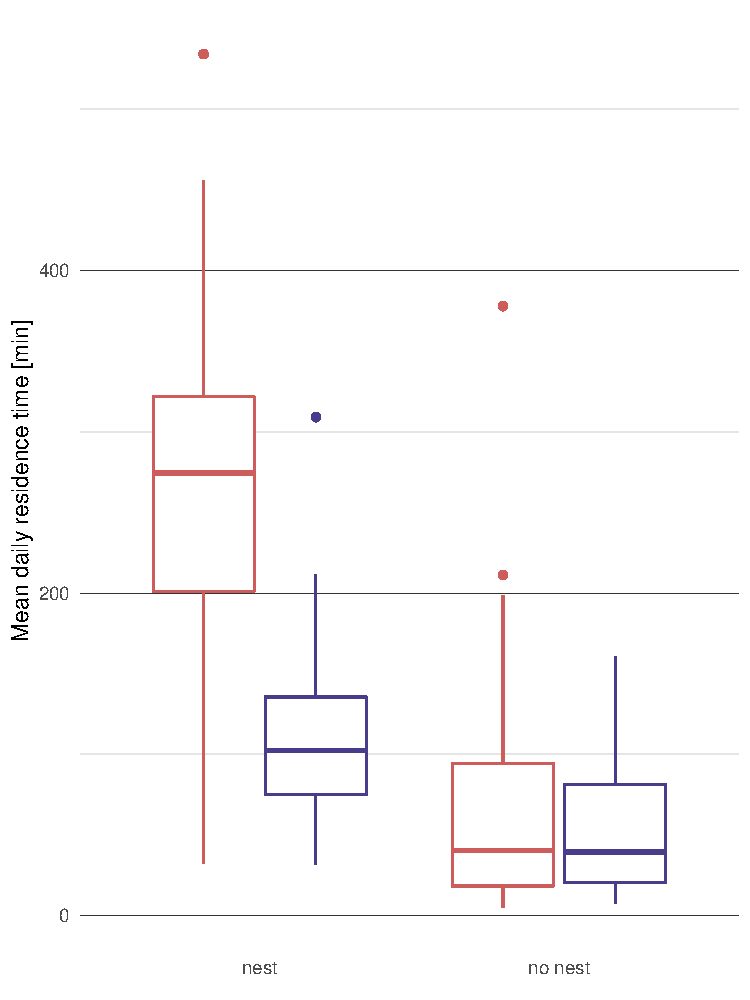
\includegraphics[width=0.4\textwidth]{figures/results/05_residence_time_sex_diff_no_legend.pdf}
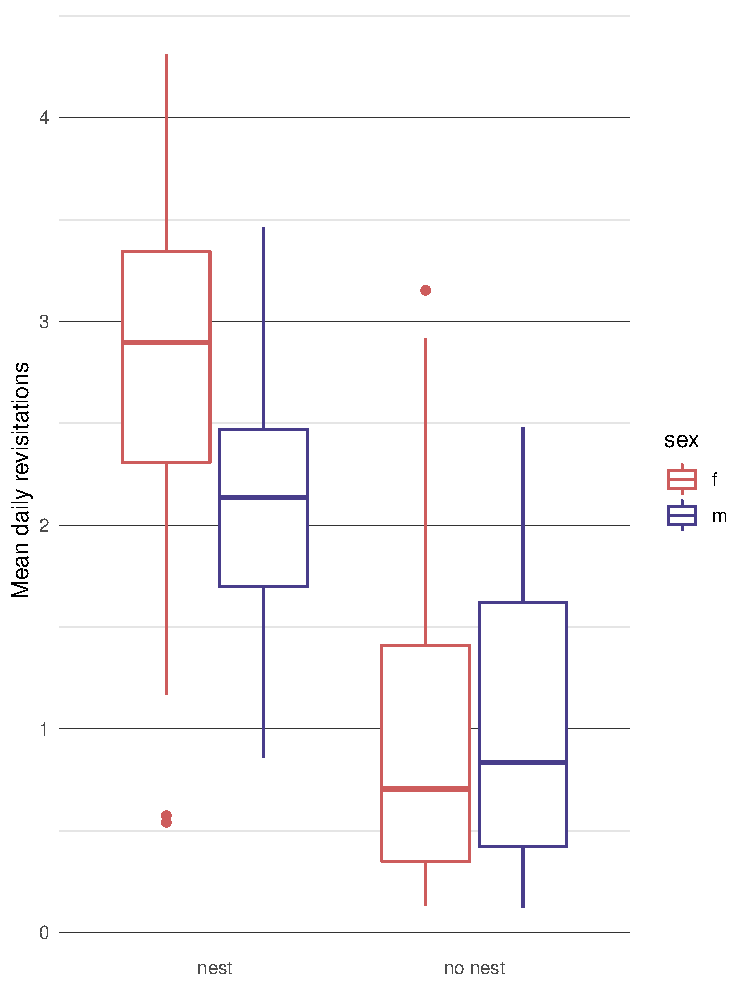
\includegraphics[width=0.4\textwidth]{figures/results/07_revisits_sex_diff.pdf}
\caption[Boxplot of birds with and without nest]{The boxplots show the difference in mean daily residence time (left) and mean daily revisitations (right) at the nest location for female (red) and male (blue) individuals with and without a nest according to the validation data.}
\label{figure:res_time_revisits_sex_diff}
\end{figure}

\vspace{1\baselineskip}

\begin{table}[H]
\begin{center}
\caption[Statistical metrics of the home range detection and the nest detection]{Overview of the statistical metrics of the home range detection and the nest detection.}
\label{table:stats_hr_and_nest}
\begin{tabular}{| p{3cm} | p{3cm} | p{3cm} |} 
\cline{1-3}
\textbf{Statistical \newline metric} & \textbf{Home Range \newline Detection} & \textbf{Nest Detection} \\
\hline
Accuracy & 77\% & 88\% \\ 
\hline
Recall & 97\% & 99\% \\
\hline
Precision & 69\% & 83\% \\
\hline
MCC & 60\% & 77\% \\
\hline
\end{tabular}
\end{center}
\end{table}



\newpage
\subsection{Accuracy of Nest Locations}
Of the 437 individuals for which a nest location was identified, for the 364 TP (the individuals that actually have a nest according to the validation data) the distance to the actual nest location was on average 71~m +/- 272~m with a median of 45~m. Of the 364 predicted nest locations, 361 were within a 1~km radius of the actual nest location. 99\% of all predicted nest locations were within a 784~m radius of the actual nest location, 95\% within a 119~m radius, and 50\% within a 34~m radius (Figure~\ref{figure:nest_dist_barplot}).

\begin{figure}[H]
\centering
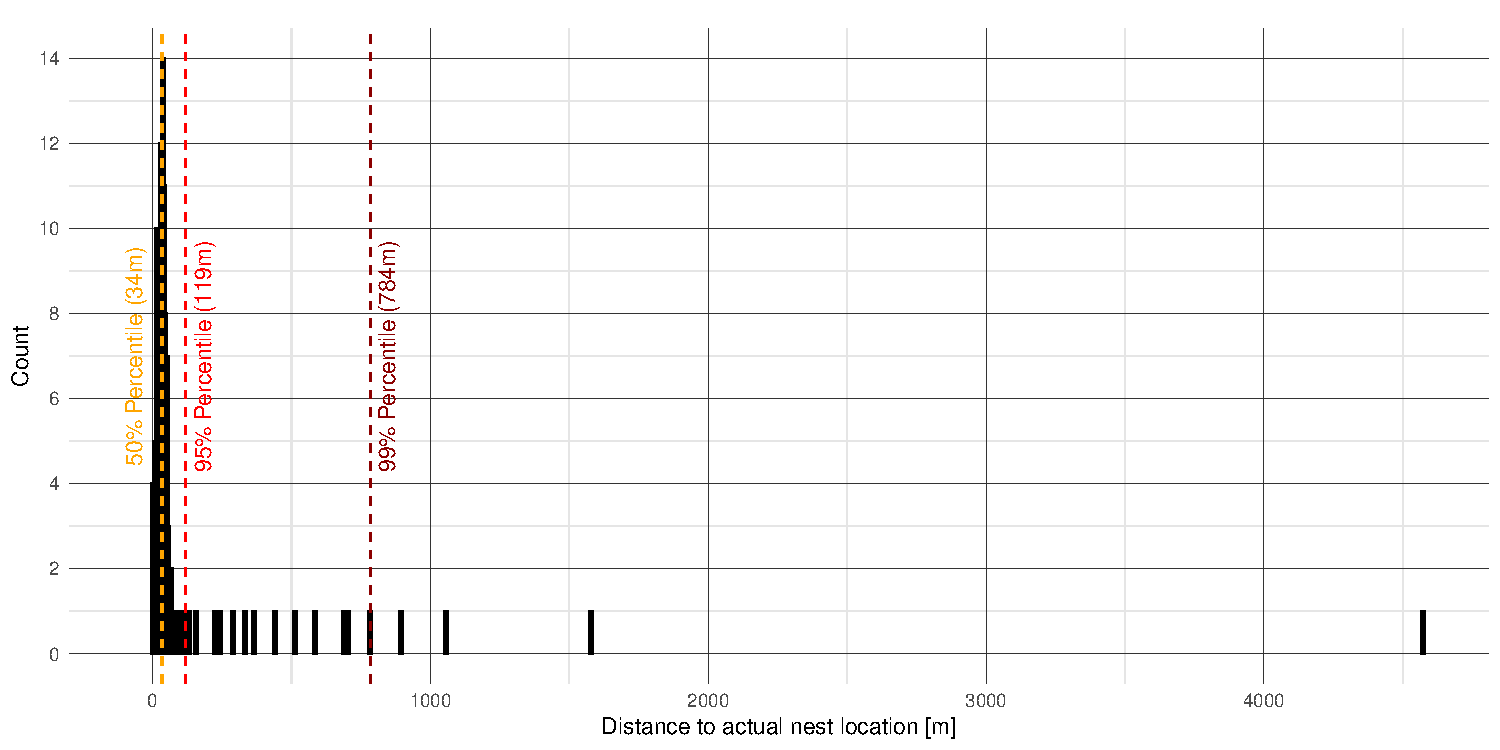
\includegraphics[width=1\textwidth]{figures/nest/nest_dist_bar.pdf}
\caption[Distances of the predicted nest locations from the actual nest locations]{Distribution of the distances of the 364 predicted nest locations from the actual nest locations.}
\label{figure:nest_dist_barplot}
\end{figure}

The distance of the predicted nest location to the actual nest location was also analysed with regard to the sex of the birds. Conducting a t-test shows with a p-value of 0.4809 that there is no significant difference between female and male individuals regarding the distance to the actual nest location.



\subsection{Brood Phase Identification}
The variable estimates of the MLRM were analysed for all three brood phases and are visualised in Figure~\ref{figure:variable_estimates} with the non-breeding phase as reference level. In the incubating phase the revisitations showed the strongest effect on the overall population, meaning that revisitations are higher during incubation compared to the non-breeding phase. Also the distance to the nest had a strong effect, decreasing during incubation. The 95\% MCP area of female individuals showed the strongest effect in the incubation phase, which decreases compared to male individuals. In the feeding phase revisitations and the 95\% MCP area increase compared to the non-breeding phase. For female individuals, the distance to the nest decreases and the residence time at the nest increases during feeding compared to male individuals. Revisitations are higher during incubating than during feeding, while the 95\% MCP area is larger during feeding than during incubating. Female individuals have a smaller 95\% MCP area usage, longer residence time at the nest and fewer revisitations at the nest location during incubating than during feeding.


\begin{figure}[H]
\centering
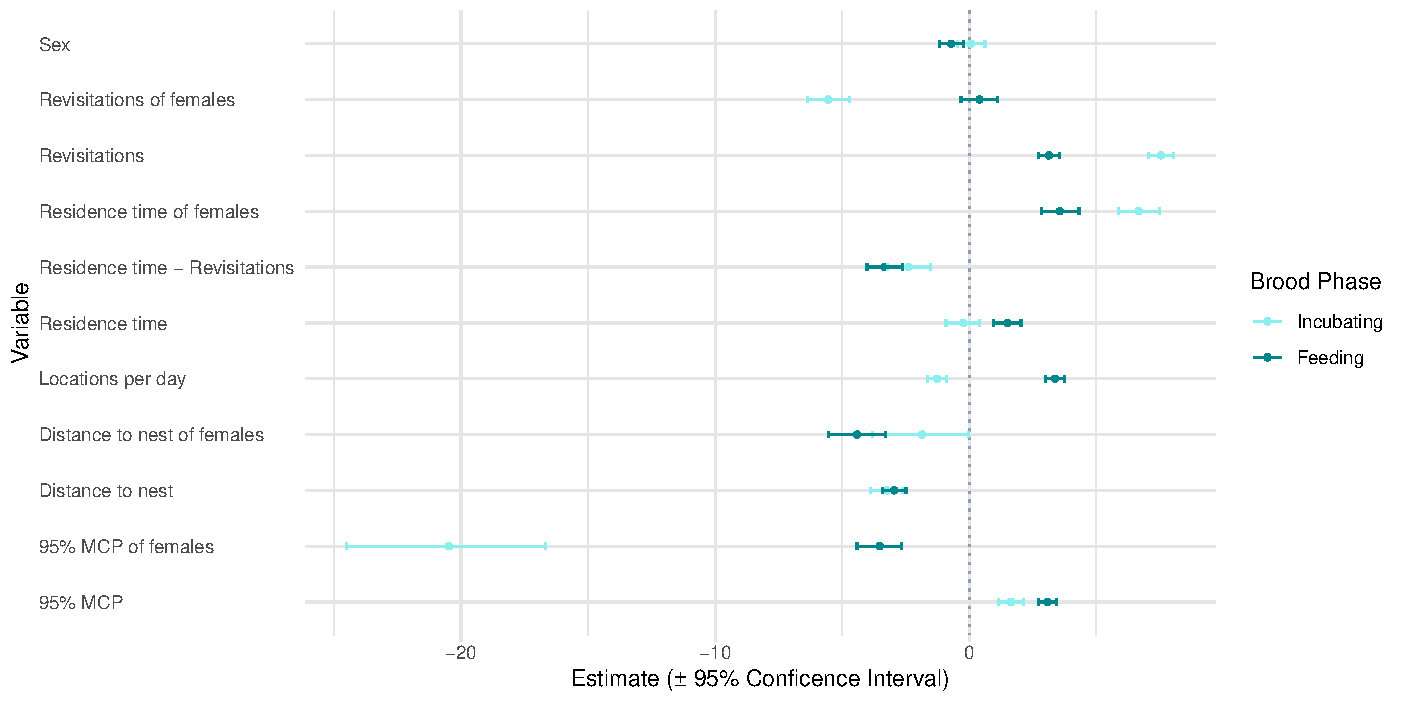
\includegraphics[width=1\textwidth]{figures/results/04_coefplot_bm_15_separated_combined.pdf}
\caption[Variable estimates of the MLRM]{Estimates of the variables used in the MLRM, shown for the two categories of incubating and feeding individuals, respectively, compared to the non-breeding category (represented as dotted line with value 0).}
\label{figure:variable_estimates}
\end{figure}


\subsubsection{Daily Predictions}
For the raw model predictions approach, 64\% of all days across all breeding cycles were correctly predicted. 49\% of all incubating days, 41\% of all feeding days and 84\% of all non-breeding days were correctly predicted. With this approach, an accuracy of 64\% was achieved. A value of 55\% was achieved for recall, 57\% for precision and 25\% for MCC (Table~\ref{table:stats_breeding_model}).

For the merged categories approach, 76\% of all days across all breeding cycles were correctly predicted. 73\% of all breeding days and 78\% of all non-breeding days were correctly predicted. With this approach, an accuracy of 76\% was achieved. A value of 73\% was achieved for recall, 78\% for precision and 51\% for MCC (Table~\ref{table:stats_breeding_model}).

For the rule-based adaptation approach, 69\% of all days across all breeding cycles were correctly predicted. 59\% of all incubating days, 46\% of all feeding days and 88\% of all non-breeding days were correctly predicted. With this approach, an accuracy of 69\% was achieved. A value of 57\% was achieved for recall, 71\% for precision and 38\% for MCC (Table~\ref{table:stats_breeding_model}).


\begin{table}[H]
\begin{center}
\caption[Statistical metrics of the different brood phase identification approaches]{Overview of the statistical metrics of the different brood phase identification approaches.}
\label{table:stats_breeding_model}
\begin{tabular}{| p{3cm} | p{3cm} | p{3cm} | p{3cm} | } 
\cline{1-4}
\textbf{Statistical \newline metric} & \textbf{Raw model \newline predictions} & \textbf{Merged \newline categories} & \textbf{Rule-based \newline adaptation} \\
\hline
Accuracy & 64\% & 76\% & 69\% \\ 
\hline
Recall & 55\% & 73\% & 57\% \\
\hline
Precision & 57\% & 78\% & 71\% \\
\hline
MCC & 25\% & 51\% & 38\% \\
\hline
\end{tabular}
\end{center}
\end{table}



\subsubsection{Brood Success Classification}
For the raw model predictions approach, 1.5\% (1 of 67) of all breeding cycles fulfill the criteria of a breeding bird, i.e. at least 28 days of incubation and 42 days of feeding of the nestlings.

For the merged categories approach, 39\% (26 of 67) of all breeding cycles fulfill the criteria of a breeding bird, i.e. at least 70 days of breeding.

For the rule-based adaptation approach, 8\% (5 of 67) of all breeding cycles fulfill the criteria of a breeding bird, i.e. at least 28 days of incubation and 42 days of feeding of the nestlings.



\subsubsection{Validation with Non-Breeding Red Kites}
Of the 73 FP cases that remained after nest detection, 34 cases had sufficient data to calculate the variables needed to apply the MLRM. Predictions of breeding behaviour were made for these 34 individuals.

For the raw model predictions approach, 48\% of all days across all breeding cycles were correctly predicted as non-breeding. 18\% (6 of 34) of all breeding cycles are falsely classified as breeding individuals.

For the merged categories approach, 41\% of all days across all breeding cycles were correctly predicted as non-breeding. 62\% (21 of 34) of all breeding cycles are falsely classified as breeding individuals.

For the rule-based adaptation approach, 56\% of all days across all breeding cycles were correctly predicted as non-breeding. 24\% (8 of 34) of all breeding cycles are falsely classified as breeding individuals.

The accuracy of the daily predictions is lower than for the breeding individuals. However, more breeding cycles are classified as successful in all classification methods.




\subsubsection{Validation with Red Kites in Thuringia}
The following results were obtained for the 28 successful broods of red kites in Thuringia:

For the raw model predictions approach, 51\% of all days across all breeding cycles were correctly predicted. 35\% of all incubating days, 65\% of all feeding days and 48\% of all non-breeding days were correctly predicted. With this approach, an accuracy of 51\% was achieved. A value of 79\% was achieved for recall, 45\% for precision and 11\% for MCC (Table~\ref{table:stats_breeding_model_pfeiffer}). 29\% (8 of 28) of all breeding cycles are correctly classified as breeding individuals.

For the merged categories approach, 72\% of all days across all breeding cycles were correctly predicted. 89\% of all breeding days and 45\% of all non-breeding days were correctly predicted. With this approach, an accuracy of 72\% was achieved. A value of 89\% was achieved for recall, 73\% for precision and 38\% for MCC (Table~\ref{table:stats_breeding_model_pfeiffer}). 86\% (24 of 28) of all breeding cycles are correctly classified as breeding individuals.

For the rule-based adaptation approach, 69\% of all days across all breeding cycles were correctly predicted. 65\% of all incubating days, 61\% of all feeding days and 79\% of all non-breeding days were correctly predicted. With this approach, an accuracy of 69\% was achieved. A value of 73\% was achieved for recall, 70\% for precision and 37\% for MCC (Table~\ref{table:stats_breeding_model}). 57\% (16 of 28) of all breeding cycles are correctly classified as breeding individuals.

The statistical metrics are similar to the breeding individuals in the Swiss data, slightly lower or higher depending on the classification method. However, more breeding cycles are classified as successful in all classification methods.

\begin{table}[H]
\begin{center}
\caption[Statistical metrics of the different brood phase identification approaches applied to red kites in Thuringia]{Overview of the statistical metrics of the different brood phase identification approaches applied to red kites in Thuringia.}
\label{table:stats_breeding_model_pfeiffer}
\begin{tabular}{| p{3cm} | p{3cm} | p{3cm} | p{3cm} | } 
\cline{1-4}
\textbf{Statistical \newline metric} & \textbf{Raw model \newline predictions} & \textbf{Merged \newline categories} & \textbf{Rule-based \newline adaptation} \\
\hline
Accuracy & 51\% & 72\% & 69\% \\
\hline
Recall & 79\% & 89\% & 73\% \\
\hline
Precision & 45\% & 73\% & 70\% \\
\hline
MCC & 11\% & 38\% & 37\% \\
\hline
\end{tabular}
\end{center}
\end{table}